\chapter{Reporting}\label{sec:Reporting}
Reporting is a core concept of Varroa.
Its purpose is to determine the results of a Varroa test and output them in a document.
The report is output in a PDF file and printed to the Commander's console.
For the latter an example is given in figure \ref{lst:ReportingOutput}.
\\
\begin{lstlisting}[caption={Excerpt from a reporting output}, captionpos=b, label={lst:ReportingOutput}, language=]
-------------- Command  Reports --------------
LifeCycle{lifeCycleId=s1.l1, clientGroupId=cg1, clientCount=100}
Connect{brokerAddress=broker.hivemq.com:1883}={
	durationSampler=[count=100, mean=228ms, stdDev=182ms, min=61ms, max=754ms],
	latenessSampler=[count=65, mean=210ms, stdDev=179ms, min=629us, max=654ms],
	failedCount=0}
Publish{pattern=topic/subtopic-[0-9], qos=1, count=1000, waitForAck=false}={
	durationSampler=[count=100, mean=10s, stdDev=7ms, min=10s, max=10s],
	latenessSampler=[-],
	failedCount=0}
Disconnect={
	durationSampler=[count=100, mean=4ms, stdDev=7ms, min=272us, max=27ms],
	latenessSampler=[count=12, mean=12ms, stdDev=4ms, min=3ms, max=17ms],
	failedCount=0}
---------------- End  Report -----------------
\end{lstlisting}

The results of a Varroa test are recorded per Action -- which means per Command execution by a MQTT Agent.
The same Actions of different clients in the same Client Group are aggregated.
This results in a single Action Report for each Action per Client Group.

\section{Actions Report}
\begin{lstlisting}[caption={Excerpt from Actions Report}, captionpos=b, label={lst:ActionReport}, language=]
-------------- Actions  Report --------------
Publish{[...]}
Publish{[...]}
Publish{[...]}
Publish{[...]}
Publish{[...]}
For{times=5}={[...]}
---------------- End  Report -----------------
\end{lstlisting}
The Actions Report allows for a finer analysis than the Report.
This is due to the fact that the Action Report does not aggregate the metrics of nested Commands like the For Command.
Instead it outputs all iterations contained in the For Command separately.
This difference becomes clear when comparing figure \ref{lst:CommandReport} and \ref{lst:ActionReport}.

\section{Commands Report}
The Action Reports are further aggregated per Command.
\\
\begin{lstlisting}[caption={Example for a Commands Report}, captionpos=b, label={lst:CommandReport}, language=]
-------------- Command  Reports --------------
Publish{[...]}
For{times=5}={[...]}
---------------- End  Report -----------------
\end{lstlisting}
The Commands Report contains aggregated metrics of every Command.
They are output in the order in which the Commands were defined in the Scenario.
With the exception of nested Commands, where the metrics of the inner Commands is output before those of the outer Command.
An example is given in figure \ref{lst:CommandReport}

\section{Reporting Architecture}\label{sec:ReportingArchitecture}
For that reason there are entities that observe the parts of Varroa that execute the Scenario.
These exist on different hierarchy levels as later explained in \ref{sec:ReportingArchitecture}. % TODO

\begin{figure}[H]
	\begin{center}
		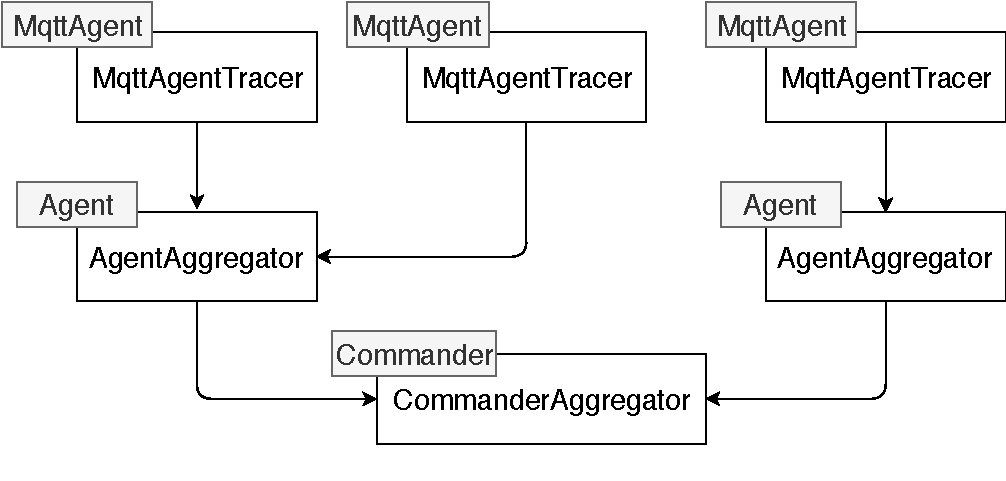
\includegraphics[scale=0.75]{Resources/PDF/ReportingArchitecture}
		\caption{Reporting Architecture}
		\label{fig:ReportingArchitecture}
	\end{center}
\end{figure}
The reporting architecture is organized in strong accordance to Varroas hierarchy.
The data flow of the report happens bottom up from the Agents to the Commander.
The reported data is recorded at the lowest level of the hierarchy namely the \emph{MqttAgentTracer} which tracks its MQTT Agents Actions.
Subsequently the \emph{AgentAggregator} receives this data and aggregates it before passing the result to the Commander.
The Commander aggregator collects the received data and then aggregates the information of all Agents and compiles it into the report.
Figure \ref{fig:ReportingArchitecture} visualizes the relationships between the components explained above.

\section{Metrics}
\subsection{Duration Sampler}
The duration Sampler gives metrics based on the duration of the executed Actions:
\begin{itemize}
	\item \textbf{count:} the amount of executed Actions.
	\item \textbf{mean:} the mean duration of the executed Actions.
	\item \textbf{stdDev:} the standard deviation of the duration of the executed Actions.
	\item \textbf{min:} the minimum duration of the executed Actions.
	\item \textbf{max:} the maximum duration of the executed Actions.
\end{itemize}
\subsection{Lateness Sampler}
The Duration Sampler reports metrics based on the lateness of expected durations of the executed Actions:
\begin{itemize}
	\item \textbf{count:} the amount of Actions whose durations exceeded the expected duration.
	\item \textbf{mean:} the mean lateness value of the actions.
	\item \textbf{stdDev:} the standard deviation of the executed Actions lateness.
	\item \textbf{min:} the minimum lateness of the executed Actions.
	\item \textbf{max:} the maximum lateness of the executed Actions.
\end{itemize}

\subsection{Failed Count}
The failed count indicates how many of the Actions were executed unsuccessfully.



